\documentclass{standalone}
\usepackage{tikz}
\usepackage{xcolor}

% colours from image (blur then colour picker)
\definecolor{0}{rgb}{0.78, 0.17, 0.125} % light red 
\definecolor{1}{rgb}{0.78, 0.42, 0.26} % orange
\definecolor{2}{rgb}{0.80, 0.81, 0.51} % light green
\definecolor{3}{rgb}{0.21, 0.27, 0.24} % dark green
\definecolor{4}{rgb}{0.235, 0.29, 0.49} % blue
\definecolor{5}{rgb}{0.255, 0.14, 0.235} % purple
\definecolor{6}{rgb}{0.475, 0.13, 0.10} % dark red
\definecolor{7}{rgb}{0.06, 0.05, 0.03} % black
\definecolor{8}{rgb}{0.40, 0.36, 0.38} % grey
\definecolor{9}{rgb}{0.98, 0.96, 0.96} % white

% fiddly command to pick the colour for the border when the inner and outer colours are the same
\newcommand{\innerline}[1]{\if#106\else\if#115\else\if#128\else\if#132\else\if#148\else\if#158\else\if#165\else\if#178\else\if#187\else\if#198\else none\fi\fi\fi\fi\fi\fi\fi\fi\fi\fi}

% The full square:
% 4/2 2/1 1/4 3/7 6/8 7/3 5/9 9/5 8/6 0/0
% 5/3 3/2 2/5 0/8 7/4 6/9 9/6 8/0 1/1 4/7
% 6/4 4/3 3/6 7/5 0/9 9/0 8/1 2/2 5/7 1/8
% 0/5 5/4 4/0 1/9 9/1 8/2 3/3 6/7 2/8 7/6
% 1/6 6/5 5/1 9/2 8/3 4/4 0/7 3/8 7/0 2/9
% 2/0 0/6 6/2 8/4 5/5 1/7 4/8 7/1 3/9 9/3
% 3/1 1/0 0/3 6/6 2/7 5/8 7/2 4/9 9/4 8/5
% 9/8 8/9 7/7 2/3 1/2 0/1 6/0 5/6 4/5 3/4
% 7/9 9/7 8/8 5/0 4/6 3/5 2/4 1/3 0/2 6/1
% 8/7 7/8 9/9 4/1 3/0 2/6 1/5 0/4 6/3 5/2

\begin{document}
    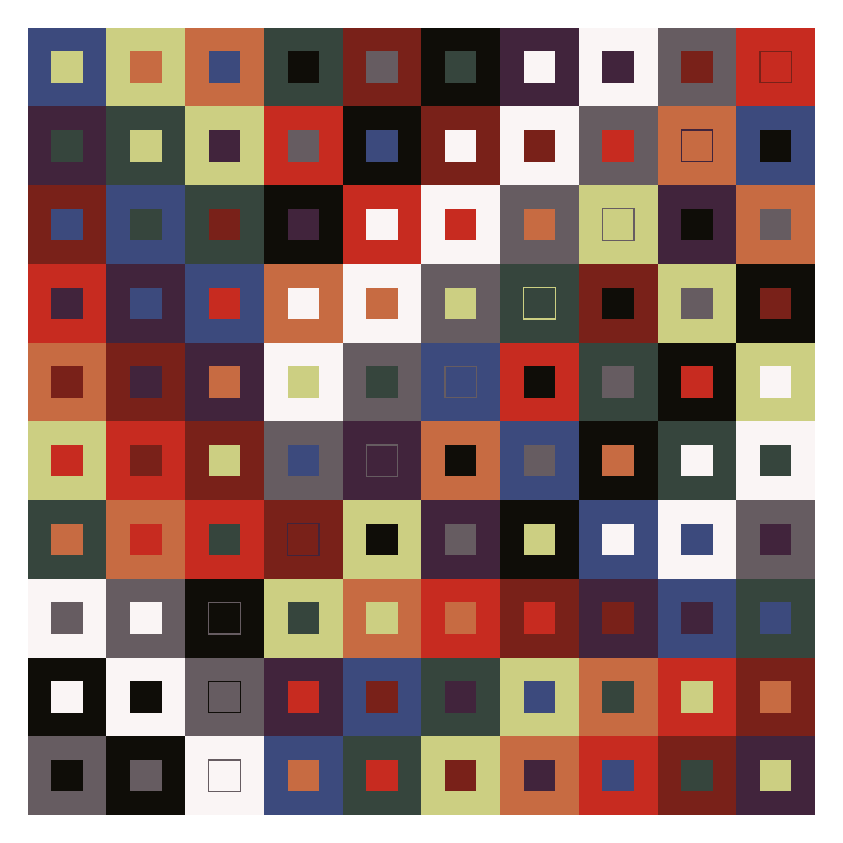
\begin{tikzpicture}
        \pgfmathsetmacro{\i}{0};
        \pgfmathsetmacro{\j}{0};
        \foreach[remember=\i as \i,remember=\j as \j] \outer/\inner in {4/2,2/1,1/4,3/7,6/8,7/3,5/9,9/5,8/6,0/0, 5/3,3/2,2/5,0/8,7/4,6/9,9/6,8/0,1/1,4/7, 6/4,4/3,3/6,7/5,0/9,9/0,8/1,2/2,5/7,1/8, 0/5,5/4,4/0,1/9,9/1,8/2,3/3,6/7,2/8,7/6, 1/6,6/5,5/1,9/2,8/3,4/4,0/7,3/8,7/0,2/9, 2/0,0/6,6/2,8/4,5/5,1/7,4/8,7/1,3/9,9/3, 3/1,1/0,0/3,6/6,2/7,5/8,7/2,4/9,9/4,8/5, 9/8,8/9,7/7,2/3,1/2,0/1,6/0,5/6,4/5,3/4, 7/9,9/7,8/8,5/0,4/6,3/5,2/4,1/3,0/2,6/1, 8/7,7/8,9/9,4/1,3/0,2/6,1/5,0/4,6/3,5/2}{ % remember is because \pgfmathtruncatemacro is local to the loop but remember brings back the previous iteration's value
            \begin{scope}[shift={(\i,\j)}]
                \draw[draw=none,fill=\outer] (0,0) rectangle (1,1);
                \if\outer\inner
                    \draw[draw=\innerline{\inner},fill=\inner] (0.3,0.3) rectangle (0.7,0.7);
                \else
                    \draw[draw=none,fill=\inner] (0.3,0.3) rectangle (0.7,0.7);
                \fi
            \end{scope}
            \if\i9
                \pgfmathtruncatemacro{\i}{0}; % CR
                \pgfmathtruncatemacro{\j}{\j-1}; % LF
            \else
                \pgfmathtruncatemacro{\i}{\i+1};
            \fi
        }
    \end{tikzpicture}
\end{document}
